\documentclass[11pt]{article}
%\documentclass{ametsoc}
\usepackage{natbib}
\usepackage[margin=1.00in]{geometry}
\usepackage{graphicx}
\usepackage{wrapfig}
\usepackage{rotating}

\title{\textbf{Modeling the Effect of Regional Climate Change in California - An Assessment of Mountain Snowpack}}

\author{Dr. Paul Ullrich (PI)}
\date{ }
   
\begin{document}

\maketitle
 
\tableofcontents

\section{Scientific / Technical / Management}
\subsection{Objectives, outcomes and recommendation}
This research proposal targets the \textbf{NSF Climate and Large-Scale Dynamics (CLD) (PD 06-5740)} with an emphasis in supporting the following objectives:
\\\\
\textit{"...processes that govern climate; the causes of climate variability and change; methods to predict climate variations; extended weather and climate predictability; numerical methods for use in large-scale weather and climate models; the assembly and analysis of instrumental and/or modeled weather and climate data; and the development and use of climate models to diagnose and simulate climate and its variations and change."}
\\\\
The \textbf{central objective} of this work is to better understand how climate change will affect water resources in California, specifically associated with mountain snowpack.  We postulate that water resources in California will shift, with a steady decline in winter snowpack, especially in lower elevation basins.  The magnitude and extent of this decline remains a key question.  In order to address this, our work will utilize a multitude of observational, climate model, and reanalysis datasets to validate a novel modeling technique, Variable Resolution Global Climate Modeling (VRGCM).

\begin{itemize}
  \item Validate and evaluate \textbf{Variable Resolution Global Climate Modeling Systems (VRGCMs)} and standard practice modeling systems in the Community Earth System Model (CESM), across a multitude of resolutions.  Additionally, we aim to compare our global/regional modeling framework to a widely used regional climate modeling system, the Weather Research and Forecasting (WRF) Model.
  \item Provide a scientifically robust assessment of the next half century (Present-2050) of changes that may affect California's hydrologic future, with specific aim at mountain snowpack. 
  \item Develop regional climate data and statistics for follow-up applications, including policymaking, water management decision making, and future research.
\end{itemize}
The proposed research is novel since it is one of the first studies in the use of VRGCMs to address real scientific questions, and the first to use the new variable resolution capability of the Community Earth System Model (CESM) to do so. Additionally, an expected outcome of our proposed research will be the development of new tools for assessing the reliability and scientific value of variable resolution modeling systems.
\subsection{Present state of knowledge}
The next century will see unprecedented changes to the climate system. The most well understood trends (such as increasing global surface temperature) are of a broad global nature and do not necessarily reflect changes on regional scales, which are key for planning on all levels. For this reason, developing a scientific understanding of changing regional climate is an unmet challenge that must be addressed. Regional climate change is particularly important to California, one of the most environmentally and agriculturally diverse regions in the world. With around two-thirds of California's developed water supply originating from the Sierra Nevada, there is growing concern that climate change will directly alter the tendencies of this natural reservoir of water.  The primary source of freshwater from this region comes in the form of winter snowpack, providing one third of California’s available water.  As global temperatures rise, snowpack is expected to decline dramatically and melt earlier in the season.  These two factors will assuredly stem late summer water flow which is integral to maintaining agricultural, environmental, and municipal water needs.  Modeling snowpack accurately requires the need for high model resolution to represent large-scale and convective snow systems, topography (with resulting orographic forcings and snow lines representations), and the overall fractal nature of snow cover and depth. To address our understanding of these features, this proposal advances the use of the next generation of modeling tools to better understand regional climate change and its effect on snowpack in California.

The climate system consists of complex interactions on a variety of scales. Changes in the climate system, which occur on the timescale of decades, inherently necessitate a global approach to ensure that these scale interactions are accurately captured by models. This requirement has made it difficult to diagnose changes to regional climate which occur due to shifts in the whole Earth system. Further, restrictions on computational cost have inherently limited the finest resolution of our uniform-resolution global climate models to around 50km, which is insufficient for resolving regional scale variability and small-scale extreme weather events. As stated in the National Center for Atmospheric Research (NCAR) 2009-2014 strategic plan, \textit{human-induced global climate change has been largely accepted as real, but information about temperature changes are not at a sufficiently fine scale for planning regional adaptation and mitigation} \citep{NCAR2009}. Consequently, the development of high-resolution regional climate simulations and associated uncertainty metrics is among the top NCAR short-term imperatives \citep{NCAR2009}. Recent advances in global Earth system modeling have focused on the development of variable resolution global climate models (VRGCMs) as a means for better understanding interactions between the global and regional scale and to improve climate projections over a limited area.  VRGCMs utilize a global coarse resolution grid which is refined over a specific area of interest; hence, these models often require only 10 percent of the computing power of uniform resolution models to resolve fine-scale features. These efforts are now beginning to come to fruition, and have led to Earth system models which both correctly capture regional-global interactions and reach the resolutions needed to understand regional climate change.   As part of its objective, this proposal addresses the need for additional development and testing of these models for tackling real scientific problems.

\subsubsection{Mountain Snowpack}
Regional climate change is particularly important to California, one of the most biologically and environmentally diverse regions in the world. The agricultural industry in California is responsible for roughly 50 percent of the nation’s fruit and vegetable production, and is particularly susceptible to extreme weather events and sudden changes in regional climate. Western mountain snowpack is a crucial reservoir for precipitation from California’s wet winters, and is an important mechanism for the gradual release of this water during the typically dry summer. In particular, summer snowmelt is an incredibly important source of agricultural water \citep{dettinger1995large, mote_declining_2005, maurer2007detection}. Recent trends in water availability have projected a potentially significant loss of agricultural water associated with loss of snow melt \citep{dyer2006spatial}. In particular, the 2013-2014 snow season was one of the driest years on record in California, with water reserves at record lows, resulting in repercussions that were felt throughout the California Central Valley agricultural communities.

Climate change directly impacts mountain snowpack via two avenues: First, warming temperatures lead to an earlier spring thaw, increasing runoff associated with spring melt and decreasing late summer water availability due to early depletion of snowpack. Second, warmer air holds more water and so leads to an increase in both large-scale and convective precipitation, although warmer temperatures also tends to favor rainfall over snowfall. Anomalous warm temperatures are particularly important in the spring at mid- to high-elevations, which would normally be below freezing throughout the winter period \citep{cayan1996interannual,stewart2009changes}. Evidence of climate change on mountain snowpack in the western US has primarily been served via empirical studies focused on April 1st measured snow depth, which has suggested there is clear evidence of a decline in snowpack throughout the western US everywhere except in the southern Sierra Nevadas \citep{mote_declining_2005}. Accumulation in this region has been attributed to an increase in the strength of the North American monsoon \citep{dyer2006spatial}. Other studies have corroborated this conclusion \citep{dettinger1995large,mote_declining_2005,knowles2006trends} and suggested that warming of the Earth’s climate will lead to a continual decline in snow resources. Further, many of these studies have demonstrated that “\textit{although the trends presented here may be partially attributable to interdecadal climate variability associated with the Pacific decadal oscillation, they also appear to result from still longer-term climate shifts}” \citep{knowles2006trends}. Current trends suggest that there will be a continued decline in mountain snowpack \citep{stewart2009changes}. Regions for which the hydrological cycle is dependent on the availability of water resources originating from melting snow or ice are expected to be particularly hard hit, with potentially dramatic effects on ecology and agriculture \citep{barnett2005potential}.

In order to obtain a robust prediction of snow water availability in the next century, global atmospheric models must be used to capture the long time scales associated with the changing climate.  However, mountain snow cover exhibits fractal-like characteristics and strong topographical dependence that makes it difficult to capture at the typical resolutions of global models. Consequently, an accurate treatment of snowpack requires grid resolution which is much finer than modern global models can produce. Hence either using dynamical downscaling to a high resolution regional model, such as the Weather Research and Forecasting (WRF) model \citep{michalakes2001development}, or a global model that captures different spatial scales, such as a VRGCM, is necessary to study modeled snowpack in a global context.

\subsubsection{Observations}
Observational datasets for snowpack metrics such as snow water equivalent (SWE), snow depth (SNOWDP), and snow cover (SNOWC) are inherently hard to capture in mountainous environments.  The fractal nature of snowpack deposits, quick shifts in elevation, angular differences in topography, alpine vegetation cover, cloud cover, and large footprint radius associated with satellite instrumentation pose challenges in resolving spatially continuous snowpack products \citep{brownandmote2009, rutter2009SnowMIP2}.  Additionally, many satellite products span less than a decade which inhibits analysis of climate patterns over decadal timeframes.  In-situ measurements help to get around some of the highlighted issues, yet they are inherently discontinuous.  Land surface models (LSM) have been used to abate the discontinuous nature of in situ observations, but may pose bias in the true state of the system.  Further, it has been shown that SWE and SNOWDP measurement error can be hard to quantify, but bias of around 10.5 percent has been seen \citep{ rutter2009SnowMIP2}.  Therefore, to try and address the multitudes of complications associated with snowpack metrics and assessment, a comprehensive blend of the aforementioned data types will be used to analyze the VRGCM climate simulations. 

There are several datasets that this study will use for validation purposes (Table \ref{t1}).  Each dataset varies in snowpack product availability, spatial and temporal resolution, map projection, and temporal range.  To provide more optimal comparisons, the aforementioned datasets will be standardized to monthly averaged, seasonally averaged (DJF), and climate averaged (25 year DJF) temporal resolutions during the assessment of the VRGCM simulations.  In order to accomplish this task, utilities from the NetCDF Operator (NCO), Climate Data Operator (CDO), and the NCAR Command Language (NCL) will be used \citep{schulzweida2007cdo,zender2006netcdf}.  

\begin{table*}[t]
\caption{Datasets, and associated metadata, used to analyze the accuracy of the Variable Resolution Global Climate Model (VRGCM) simulations}\label{t1}
\begin{center}
\begin{tabular*}{\textwidth}{@{\extracolsep\fill}lcccccccc}
\hline
$Datasets$ & $Snowpack  Product$ & $ Spatial  Resolution$ & $Temporal  Resolution$ \\
\hline
 CMC & SWE, SNOWDP & 24km & Daily\\
 DAYMET & SWE & 1km & Daily \\
 MODIS/Terra & SNOWC & 5km & Monthly \\
 SNOTEL/Snow Course & SWE, SNOWDP & Point Source (24 stations) & Daily \\
 NARR & SNOWDP, SNOWC & 32km & Daily \\
 NCEP (CFSV2) & SWE, SNOWDP, SNOWC & 35km & Daily \\
 Uniform CESM & SWE, SNOWDP, SNOWC & 25km & Daily \\
 WRF & SWE, SNOWDP, SNOWC & 27km, 9km & Daily \\
\hline
\end{tabular*}
\end{center}
\end{table*}

The Canadian Meteorological Centre (CMC) SNOWDP dataset is comprised of surface synoptic observations and meteorological aviation reports from the World Meteorological Organization’s information system.  CMC derives SWE values using the aforementioned SNOWDP measurements and look-up tables for snow density values \citep{brown2003gridded}.  The DAYMET dataset provides SWE estimations from interpolated meteorological stations.  The interpolated station data is then extrapolated, using a truncated Guassian weighting filter, to create a high resolution gridded output \citep{thornton2012daymet}.  The Moderate Resolution Imaging Spectroradiometer (MODIS) satellite dataset provides SNOWC using a snow mapping algorithm with a Normalized Difference Snow Index (NDSI) \citep{salomonson2006development}.  The NDSI is used to distinguish between snow and other features (such as cloud cover) by using visible and short wave near IR spectral bands \citep{salomonson2006development}.  The SNOwpack TELemetry (SNOTEL) in situ dataset is comprised of 24 automated observational stations spread throughout the Sierra Nevada mountain range measuring SNOWDP and SWE \citep{serreze1999characteristics}.  The areal extent of the SNOTEL stations range from 38.07$^{o}$ to 42.99$^{o}$ latitude by -120.79$^{o}$ to -119.23$^{o}$ with an average elevation of 2343.45 meters.  In addition to maintaining the SNOTEL automated station dataset, the Natural Resources Conservation Service (NRCS) also takes in situ snow course measurements of SNOWDP and SWE by trained observers at 32 permanent sites.  The measurements are taken during the first of every month in January through May along a 305 meter long transect line, usually in small meadow areas, with an average elevation of 2293.01 meters.  The North American Regional Reanalysis (NARR) dataset provides monthly averaged SNOWDP and SNOWC output variables using a high resolution atmospheric model (Eta Model) forced by a Regional Data Assimilation System (RDAS) \citep{mesinger2006north}.  The other reanalysis dataset (NCEP - CFSV2) that will be used is a recently updated (2013) version of its predecessor (2004).  The NCEP dataset provides improved two meter surface temperature, MJO, and SST forecasts while upgrading overall performance in seasonal/subseasonal forecasting results, compared to its predecessor \citep{saha2014ncep}. NCEP has also been advised for use by decision makers in the water management and agricultural fields \citep{saha2014ncep}.  Two 0.25$^{o}$ uniform resolution (spectral element and finite-volume dynamical cores) CESM datasets will be used to intercompare with the VRGCM simulations too.  These two simulations were conducted by a team at Lawrence Berkeley National Laboratories (LBNL). To provide added benefit to the proposal, we will compare the VRGCM simulations to a pair of regional climate model (RCM) simulations too.  A pair of simulations will be conducted at UC Davis using an “out of the box” version (V3.5.1) of the Weather Research and Forecasting (WRF) model, a widely used RCM.  The simulations will use a multi-resolution domain with a coarse resolution of 27km and a finer resolution domain of 9km situated over the western USA (centered on the Sierra Nevada).  Both WRF domains provide SWE, SNOWDP, and SNOWC output variables.

\subsubsection{Strengths of the Investigation Team and Ongoing Work}
The PI has extensive first-hand experience with atmospheric model development, having developed a global shallow-water model \citep{ullrich2010high}, a regional atmospheric modeling system \citep{ullrich2012operator} and a fully 3D non-hydrostatic dynamical core \citep{ullrich2012mcore}. Further, he has worked on adaptive mesh refinement and quasi-uniform grid geometries in extensive detail \citep{collins2013nonhydrostatic}. He is heavily involved in national collaborations on climate projects, and is an organizer on a number of sessions and workshops which are related to atmospheric modeling. In addition, he is closely affiliated with ongoing climate research efforts at Lawrence Berkeley National Laboratory (LBNL) and NCAR. He is currently working on the question of extreme weather detection and attribution for extratropical cyclones and pressure blocking events leading to heat waves along with students Marielle Pinheiro and Josephine Fong. As part of a summer internship they are working jointly with the PI, Dr. Michael Wehner (LBNL) and others on the LBNL climate research team (Bill Collins, Dan Martin, Daıthı Stone, Prabhat, and others).

Dr.  Shu-Hua Chen (UC Davis) has extensive experience with using WRF for regional atmospheric modeling and so will be a valuable collaborator towards the completion of this project. She will be assisting with the use of WRF for simulating the snowpack, as well as coupling WRF to the CESM ensemble data.

The PI and his collaborating team are uniquely positioned to conduct multi-model ensemble intercomparisons using a suite of cutting-edge atmospheric models. This award will not only serve as a springboard for the PI’s future career, but will also provide a framework for future variable resolution intercomparison studies and an improved understanding of hydroclimate effects facing California.

\subsection{Variable Resolution Global Climate Modeling (VRGCMs)}

The Community Earth-System Model (\citet{hurrell2013community}, CESM) is a state-of-the-art Earth modeling framework developed at NCAR, consisting of atmospheric, oceanic, land and sea ice components. This framework has been under development for nearly two decades, and has been used heavily in better understanding the effects of global climate change. The Community Atmosphere Model (CAM, the atmospheric component of CESM) is further broken into two components: the dynamical core, which solves the 3D primitive equations of motion for the atmosphere, and the physics parameterization suite, which incorporates processes that occur on scales below the model grid scale. Because of its modular nature, CAM currently allows for switching between four dynamical cores, including the finite-volume, semi-Lagrangian, Eulerian and spectral element dynamical cores, with work underway for the inclusion of others in the near future. Of these four, only one dynamical core has variable resolution capability, namely the CAM spectral element (SE) dynamical core (CAM-SE).

The spectral element method has several important properties including parallel scalability, flexibility and accuracy, that make it a desirable choice for modeling atmospheric dynamics. The spectral element dynamical core \citet{fournier2004spectral, taylor2010compatible} is now the default dynamical core in CAM and so is a supported platform for scientific research. Recently CAM-SE has added variable resolution support which allows for coupled climate simulations in CAM on a variable resolution atmospheric mesh. The mesh must be conformal, so each edge is shared by exactly two quadrilateral spectral elements. A couple examples of the meshes that we will use are depicted in Figure \ref{f1}, which shows smooth refinement over North America from a global resolution of 1.0$^{o}$ to a refined region with 0.25$^{o}$ (right) and 0.125$^{o}$ (left) grid spacing over the US west coast.  We have also incorporated variable resolution grids into the land surface model of CESM (CLM).  This is a new breakthrough that will unify the two meshes in both models and eliminate potential grid to grid interpolation issues.  There have been recent modeling efforts using variable resolution support in CAM-SE including both short-term weather forecasting and longer-term climate forecasting, with an interest in obtaining hurricane counts in the Atlantic basin \citep{zarzycki2014using}.

\begin{figure}
  \begin{center}
  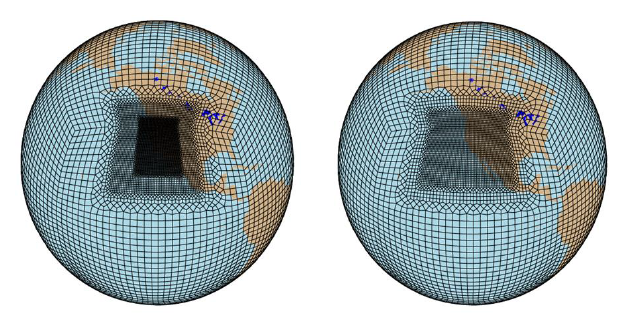
\includegraphics[width=0.75\textwidth]{14kmand28kmgrids}
  \caption{\label{f1}The two Variable Resolution Global Climate Model (VRGCM) grids (14km, left, and 28km, right) implemented into the Community Earth System Model (CESM) for this study.  Both grids base resolution are 1$^{o}$ cubed-sphere.  Over the western USA, a halving of resolution in each distinct domain region occurs with the inner most domain featuring a 14km resolution (left) and 28km resolution (right).}
  \end{center}
\end{figure}

As shown by the most recent snow model intercomparison project (SnowMIP2), a comprehensive assessment of 33 snow models with varying complexity and intended development purpose, no model was shown to perform best across a range of discrete locations in the Northern Hemisphere \citep{rutter2009SnowMIP2}.  Further complications arose in the intercomparison project when canopy interactions were assessed as models performed differently with vegetated and non-vegetated environments.  \citet{rutter2009SnowMIP2} found that a key indicator of more optimal performance in a snow model is its ability to characterize vegetation cover, winter temperature characterization, and performance across a multitude of variables (e.g. snow cover, snow depth, and snow water equivalent).
    
CLM (version 4.0) utilizes a grid cell by grid cell specification routine that breaks each model cell into a unique combination of land unit types including: glacier, lake, urban, vegetated, and wetland \citep{lawrence2011parameterization}.  The vegetated component of the grid cell is further broken down into various soil types which are then characterized by 15 unique, plus non-vegetated, Plant Functional Types (PFTs) \citep{lawrence2011parameterization}. CLM4 PFTs include: five evergreen species and six deciduous species for temperature, boreal, and tropical climates, three grasses for arctic and non-arctic climates (with C-3 and C-4 variations) and a few staple cereal crops \citep{lawrence2011parameterization}.  PFT cover is derived from the Moderate Resolution Imaging Spectroradiometer (MODIS) satellite data at 0.5$^{o}$ resolution with canopy heights for each of the PFTs assumed to be constant and canopy diameters ranging from 0.5 meters (crops, grasses, and shrubs) to 35 meters (trees) \citep{lawrence2011parameterization}.  

As discussed previously, PFT types and percent cover of PFTs within each vegetated land-unit play a crucial role in shaping snowpack trends. This is because the interaction between the canopy and snowpack are PFT specific for biogeochemical, radiative, and hydrological processes including: interception, throughfall, canopy drip, water removal via transpiration, and optical property interactions based on leaf angle and specific PFT \citep{lawrence2011parameterization}.  Therefore, CLM4 provides a relatively complex representation of snowpack and its biogeophysical interactions within a GCM framework, lending itself well to this study.   A higher resolution dataset for PFT type would have been beneficial for this study, to capitalize on the higher resolution (less than 0.5$^{o}$) VRGCM grids implemented into both CAM5 and CLM4, however none were found.

The parameterizations of snowpack within CESM are based primarily on work done by \citet{anderson1976point}, \citet{jordan1991one}, and \citet{yongjiu1997land}. These parameterizations characterize several important state variables for snowpack including: the mass of water, mass of ice, snowpack layer thickness, temperature profile of the snowpack layer, black carbon and mineral deposition, and snowpack aging and optical properties \citep{lawrence2011parameterization}. Through the characterization of these state variables, in numerically discretized equations, a five layer snow model with dynamic compaction, water transfer, and energy transfer was created \citep{lawrence2011parameterization}, the SNow and Ice Aerosol Radiation (SNICAR) model.  The SNICAR model replaced the CLM3 snow model which was used in the SnowMIP2 intercomparison project.  This has resulted in a much more complete representation of snowpack, and its tendencies, than its predecessor used in SnowMIP2.

\subsection{Research Tasks}
This proposal incorporates both a computational and a scientific focus. The computational focus will utilize a suite of modeling tools to improve model resolution over California, and provide an evaluation on the effectiveness of these tools for capturing small-scale features. Studies of enhanced resolution via dynamical downscaling (using the WRF regional model) and variable resolution modeling using the fully integrated VRGCM in CESM will be performed. The scientific focus will use the simulation data to determine whether the dynamically downscaled model and VRGCMs are able to capture the 20th century trend in snowpack loss and and isolate model predictions on the future behavior of these snowpack fields.

The tasks required for this project will be completed in three stages: In the first stage, control simulations will be run over the 1980-2005 time period. Snowpack indicators will then be compared against the bevy of observational products highlighted above to verify consistency between the modeled climatology and observations. In the second stage, the VRGCMs will be used to execute a similar set of simulations over the same time period and the results compared against the control simulation to determine any inherent differences in the behavior or predictive capability of the VRGCMs versus the dynamically downscaled WRF simulation. In the third stage, the VRGCM simulations will be extended to a predictive ensemble over the 2025-2050 time period using both Climate Variability and Predictability (CLIVAR)-type Atmospheric Model Intercomparison Project (AMIP) forcings (prescribed sea-surface temperatures) and fully coupled global atmospheric simulations with a fully coupled ocean. Results from the predictive simulations will be compared to the control simulations to determine the mean behavior and variability of the snowpack under future warming scenarios.

\subsubsection{WRF Simulations (1980-2005)}
An ensemble of control simulations will be constructed using the limited area two-way WRF model run over the US west coast at high resolution (10km resolution at the highest refinement level, with additional nested refinement levels at 20km and 55km). The outer domain will approximately cover 15N to 60N and 150W to 100W. Initially an ensemble of 10 perturbed initial condition runs will be used, with additional simulations added as needed. ERA reanalysis data will be used for the initial conditions, lateral boundary conditions and prescribed sea-surface temperatures. The period of integration will be 1980-2005 with the WRF simulation nudged to the reanalysis data to reduce disagreement between ERA and WRF. Snow products such as snowdepth (snowpack), snow water equivalent, surface snow cover will obtained from the output data.  These model outputs will then be compared over the simulation period with all of the observational datasets highlighted above, so as to quantify the quality of the coupled regional-global model results. Precipitation results, which can be very sensitive to model and topographical resolution, will also be compared with rain gauge data to verify consistency with historical observations.  Additionally, surface energy budgets and temperature profiles will be assessed to identify behavioral traits in snowpack tendencies.

Once model output is obtained, correlations between observational products and model outputs will be computed and compared at both the regional and grid point scale to determine any intrinsic biases in the simulation results. Specifically, these biases may be due to particular sensitivities in the model, such as issues due to unresolved topographical forcing or in the physical treatment of precipitation. The use of an ensemble of simulations is particularly useful for determining the statistics of the climatology generated in each case, including the mean and variance associated with each of the variables of interest.

\subsubsection{VRGCM Assessment Simulations (1980-2005) and Tuning}
An analogous approach to section 1.4.1 will now be applied  for  the  CESM  (CAM-SE and CLM4.0) using built-in support for variable resolutions.  Specifically, these models will be run with a 100km base resolution refined to 14 and 28km regional resolution. For the CESM model a multi-level refined grid, shown in \ref{f1}, will be used with three levels of refinement from a background 110km (1$^{o}$) resolution. The region of high resolution will be chosen to closely correspond to the region of refinement for the WRF model.  One experiment will also examine whether simulation results can be improved by nudging towards the reanalysis data over the duration of the integration.

Again the assessment period will be 1980-2005, and both models will be driven using global prescribed SSTs (in correspondence with the AMIP protocol). Model results will be compared over the 1980-2005 time frame with snowpack observational products. Further, results from the VRGCMs  will  be  compared against the ensemble WRF simulations. This procedure will again allow quantification of biases associated with the VRGCMs and if any additional tuning is required to produce more realistic simulation results.  Specifically, topographical smoothness has been identified as one substantial source of uncertainty in these simulations, especially for the purposes of computing statistics related to snowpack.

\subsubsection{VRGCM Predictive Simulations (2025-2050)}
Once the VRGCM CESM simulation has been assessed over the 1980-2005 time period, the next step is the use of this model for active prediction of future snowpack. To limit the computational cost of the predictive model and allow for additional experiments, only the 2025-2050 simulation period will be considered initially. A suite of experiments will be pursued, as listed in Table 1 using climate forcings derived from the Intergovernmental Panel on Climate Change (IPCC) fifth assessment report Representative Concentration Pathways (RCP), as well as present day control simulations and CLIVAR-type 2xCO2 experiments. Sea-surface temperatures will either use present day values following the AMIP framework, modified sea surface temperatures (+2 degrees warmer) or will be obtained online via a fully coupled model ocean.

\begin{table}[t1]
\begin{center}
\caption{Predictive experiments for the VRGCM simulation over the 2025-2050 simulation period}
\begin{tabular}{|l|r|r|} \hline
Experiment & Climate Forcing & Sea-Surface \\\hline
Control & Present day & Present day (AMIP) \\
2xCO2 & 2xCO2 & Present day (AMIP) \\
SST+2 & Present Day & SST+2 (AMIP) \\
2xCO2, SST+2 & 2xCO2 & SST+2 (AMIP) \\
8.5-FULL & RCP8.5 & Fully coupled \\
2.6-FULL & RCP2.6 & Fully coupled \\\hline
\end{tabular}
\end{center}
\end{table}

Using the ensemble of model simulations, snowpack information will be assessed for both mean and variance over the duration of the simulation. Further, the spatial dependence of these quantities will be used to provide local assessments in Northern California, the Sierra Nevadas, and Southern California regions.

\subsubsection{Data Publication}

Data from both the WRF run and VRGCM runs will be post-processed and made available for future use via the Earth System Grid \citep{williams2009earth}. This archive allows for public access to model output from all simulations and consequently allows for these results to be leveraged for future study.  The data will be post-processed and made available in different temporal resolutions (i.e. daily, monthly, seasonal, and climate) using the Climate Data Operators (CDO) and NetCDF Operators (NCO) \citep{schulzweida2007cdo,zender2006netcdf}. 

\subsubsection{Computational Requirements}
Benchmark tests have been run to verify the computational capacity of the UC Davis computing cluster for VRGCM simulation. Refining the Atlantic hurricane basin to 12.5km resolution over a 110km base resolution has led to an approximate assessment of one month of computing time for a thirty year simulation with prescribed sea surface temperatures on 768 processor cores using CESM. The fully coupled simulations are slowed by the requirement to simulate the ocean, but only a limited number of fully coupled simulations will be required. These simulations have been projected to require roughly two months of computing time over the forty year prediction time. Multiple simulations will also be run in parallel to improve computational throughput.

\textbf{UC Davis}:  This project requires computational resources for implementation and testing of software over the course of the project. The University of California, Davis has recently invested in building a campus-wide computing cluster for the advancement of scientific research in the environmental sciences, of which a significant portion was provided as part of the PI’s start-up package. Consequently the PI and his research team will have high-priority access to this cluster, with over 1,500 processors, including full-time technical support from the campus computing team. A laptop for the graduate student researcher is also provided by the PI’s start-up package.

\subsubsection{Plan of Work}
The PI, Dr. Paul Ullrich, will be the primary administrator for the project, and will be responsible for managerial and administrative decisions, including planning, scheduling and oversight of research tasks, plus reporting of technical progress. He will be the primary contact on this project and will be the point of engagement for project collaborators and their teams. He will further be responsible for ensuring that sufficient computational resources are available for continued progress on the project. The majority of the requested funds will be used to pay for one full-time Graduate Student Researcher (GSR) who will pursue this research as part of their Ph.D. research. The GSR will be advised full-time by the PI at UC Davis. In addition, funding will be used to reimburse the PI for one month of salary, which will be used to fund a eight percent commitment of effort to support the GSR on this work. The PI and GSR will meet once per week to discuss the progress and status of the project. Milestones for this project are given below:

\begin{itemize}
  \item \textbf{Year 1} - Intercomparison of metrics for snowpack, couple ERA data to WRF, completion and assessment of coupled WRF simulations, installation and testing of VRGCM on UC Davis cluster, and implementation of post-processing scripts
  \item \textbf{Year 2} - VRGCM assessment simulations, scripts for comparison of modeled (VRGCM and WRF) outputs and observational datasets, and implementation of VRGCM predictive simulation framework
  \item \textbf{Year 3} - VRGCM predictive simulations (control, CLIVAR, RCP), assessment of predictive simulation results, post-process and publishing of simulation data, project wrap-up, and submit final report
\end{itemize}

We expect results and research progress will be presented at regular scientific meetings, including meetings of the American Geophysical Union (AGU) and the American Meteorological Society (AMS). This work will also be presented at the CESM annual working group meeting and CESM atmospheric working group meeting. We further anticipate that we will publish at least one peer-reviewed article in each year.

\section{References}
\bibliographystyle{ametsoc2014}  
\bibliography{references_NSFsnowpackproposal}
 
\section{Biographical Sketch}

\section{Current and Pending Support}

\section{Statements of Commitment / Work}

\section{Budget Justification}
Expected Award Instrument:  Grant

\subsubsection{Inflation}
The inflation rate is assumed to be three percent per year on salaries and travel expenses.

\subsubsection{Salaries}
\textbf{Principal Investigator} -
The principal investigator [Paul Ullrich] will be reimbursed for one month of summer expenses starting in FY15, following the standard UC Davis salary track for fiscal year faculty. This rate amounts to \$8201 per month in FY15 and \$8437 per month in FY16. The PI is already funded for summer salary in FY14 via a UC Davis start-up award.
\\\\
\textbf{Graduate Student Researchers} -
One graduate student researcher [Alan Rhoades or Xingying Huang] (GSR4; nine months at 48 percent, three summer months at 100 percent) will be given a stipend each year as part of this project. The student will be from the graduate group in atmospheric science at UC Davis. This project will be conducted as part of his/her Ph.D. degree. The monthly salary rate for a GSR4 is \$3775 for July 2014 through June 2015, with inflation applied in subsequent years.

\subsubsection{Fringe Benefits}
Fringe benefit rates for those working on the project are standard UC Davis rates, as follows: Faculty summer salary (17 percent in Year 2, 18 percent in Year 3) and Graduate Student Researcher (1.3 percent).

\subsubsection{Travel and Living}
The budget includes domestic flight costs to major conferences, including the American Meteorological Society (AMS) annual meeting and American Geophysical Union (AGU) annual meeting. Specifically, the budget includes one trip per year for the PI and student, with some additional funding expected to be available from UC Davis. Travel costs and miscellaneous expenses are estimated at \$300 for the AGU conference which is traditionally held in San Francisco, CA and \$600 for the AMS conference which varies by location through the continental United States. The domestic subsidence rate is estimated to be \$180 per day (which includes hotel and per diem meal costs) plus local transportation costs of \$30 per day. Registration fees are estimated at \$600 per year.

\subsubsection{Other Direct Costs}
\textbf{Publication Costs}
Publication costs are incurred from publication of work produced by this project. The estimated cost is \$1200 per year for publication costs.
\\\\
\textbf{Software  Licenses}
Software license charges include a one time \$145 charge for the mathematics software package Maple and one \$165 / year charges for the software package Matlab. These software packages will be used by the student for data processing, intercomparison and modeling. Other software, such as Microsoft Office, is available for free via a UC Davis license.
\\\\
\textbf{Other Direct Costs:  Tuition}
The UC Davis 2014-15 estimated graduate California resident student fees are \$5905 per quarter, with no tuition paid during the summer quarter. Tuition is expected to increase by 10 percent for each academic year thereafter. This amounts to \$17,715, \$19,487 and \$21,436 for years 1, 2 and 3.

\subsubsection{Indirect Cost}
Indirect costs are charged by UC Davis on salaries, supplies, travel and hosting at a rate of 55.5 percent, 56.5 percent and 57 percent for years 1 through 3.

\subsubsection{Personnel and Work Effort}
\textbf{Paul Ullrich} - Eight percent effort

\end{document}